% Three-page editorial sample. Not the final internship report.
\documentclass[a4paper,11pt,oneside,headings=normal]{scrreprt}
\usepackage[left=25mm,right=23mm,top=23mm,bottom=23mm]{geometry}
\usepackage{fontspec,unicode-math,microtype,graphicx,booktabs,tabularx,xcolor,listings,hyperref,scrlayer-scrpage}
\setmainfont{LibertinusSerif}[Extension=.otf,UprightFont=*-Regular,ItalicFont=*-Italic,BoldFont=*-Bold,BoldItalicFont=*-BoldItalic]
\setsansfont{LibertinusSans}[Extension=.otf,UprightFont=*-Regular,ItalicFont=*-Italic,BoldFont=*-Bold]
\setmathfont{LibertinusMath-Regular.otf}
\definecolor{Navy}{HTML}{173A5E}\definecolor{Teal}{HTML}{2E6F73}\definecolor{Ink}{HTML}{20242A}\definecolor{Grey}{HTML}{F3F5F7}
\color{Ink}\hypersetup{colorlinks=true,urlcolor=Teal,pdfauthor={Ali Erkan Ocaklı},pdftitle={RobustCluster-Aβ: editorial preview}}
\setkomafont{disposition}{\sffamily\bfseries\color{Navy}}
\clearpairofpagestyles\ihead{\sffamily\small RobustCluster-Aβ}\ohead{\sffamily\small Editorial sample / 7 October 2026}\cfoot*{\pagemark}\pagestyle{scrheadings}
\setlength{\parindent}{0pt}\setlength{\parskip}{6pt}\setlength{\emergencystretch}{2em}
\lstset{basicstyle=\ttfamily\small,backgroundcolor=\color{Grey},breaklines=true,columns=fullflexible,keepspaces=true,showstringspaces=false,frame=none}
\newcommand{\AnalysisRun}{20261007T104141-f0143175}

\begin{document}
\begin{titlepage}
{\sffamily\large University of Messina\par}
{\sffamily Data Analysis L-31\par}
\vspace{15mm}
{\sffamily\small\color{Teal} CURRICULAR INTERNSHIP REPORT\par}
\vspace{6mm}
{\sffamily\fontsize{32}{37}\selectfont\bfseries\color{Navy}RobustCluster-Aβ\par}
\vspace{5mm}
{\sffamily\LARGE Reproducible analysis of\par amyloid-β40 conformational descriptors\par}
\vspace{5mm}
{\large Scientific code audit, sampling diagnostics\par and feature-space sensitivity\par}
\vspace{10mm}
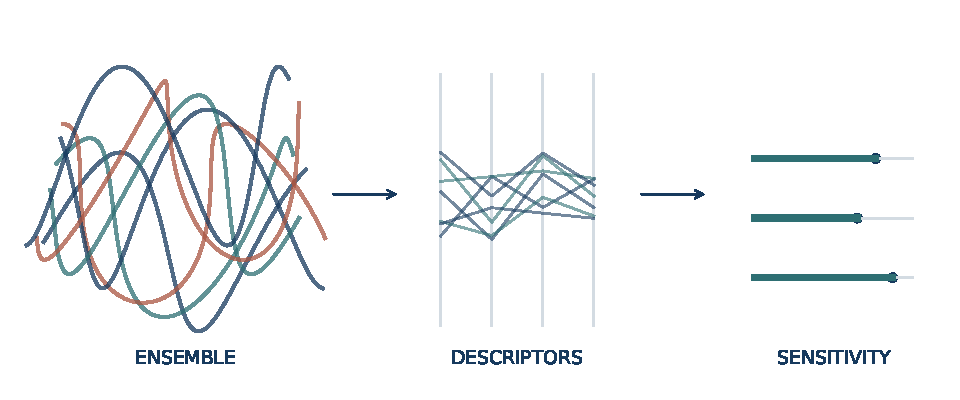
\includegraphics[width=\textwidth]{cover_concept.pdf}
{\small\itshape Conceptual ensemble-to-analysis illustration. Lines and marks are schematic; they are not molecular coordinates or computed cluster results.\par}
\vfill
\begin{tabularx}{\textwidth}{@{}lX@{}}
Student & Ali Erkan Ocaklı\\[2mm]
Matricola & 555012\\[2mm]
Internship contacts & Andrea Ciccolo; Valeria Conti Nibali\\[2mm]
Academic year & 2025–2026
\end{tabularx}
\vspace{8mm}
{\small\sffamily Design sample · cover and two internal pages\par}
\end{titlepage}
\section*{Does removing SASA change the partition?}
Radius of gyration and solvent-accessible surface area describe related aspects of peptide conformation. Their correlation motivates a sensitivity test, but correlation alone does not establish that either variable can be discarded. Here the same observations are clustered with four descriptors and again after removing SASA.

A fixed sample of 1,000 frames per replica was used to fit standardization and Gaussian mixture models. Five initializations were examined for each component count from two to six. Assignments were compared on all 300,003 frames, including those used for fitting. This is a descriptive comparison of biased samples, not a held-out prediction test.

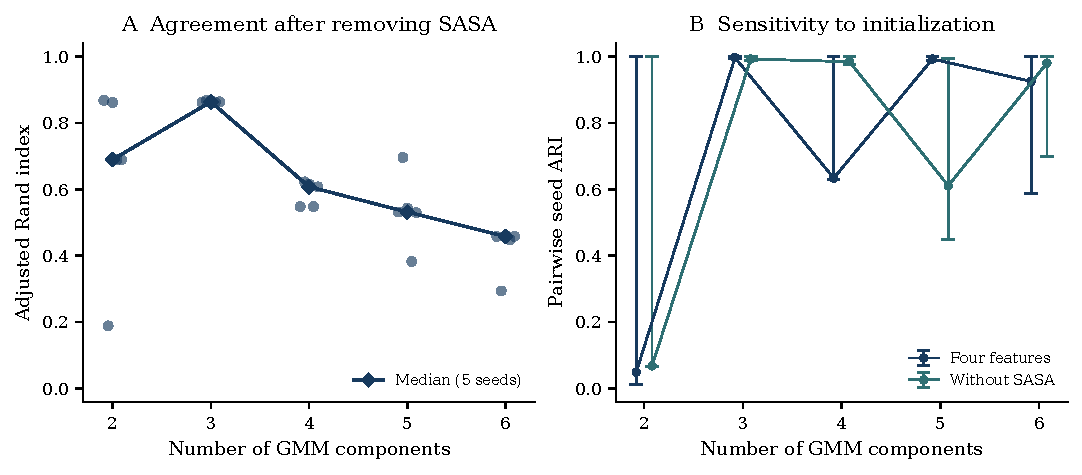
\includegraphics[width=\textwidth]{gmm_sensitivity.pdf}
{\small\textbf{Figure A. Representation and initialization sensitivity.} Left: four-feature versus three-feature agreement, with one dot per seed and a line through the median. Right: pairwise seed agreement within each feature space; bars span the observed minimum and maximum across ten comparisons. Bars are not confidence intervals. Source: successful run \texttt{\AnalysisRun}.\par}
\vspace{3mm}
\begin{center}
\begin{tabular}{@{}crr@{}}\toprule Components & Median ARI, four vs three features & Observed range\\\midrule
2 & 0.690 & 0.188--0.868 \\
3 & 0.864 & 0.862--0.868 \\
4 & 0.607 & 0.548--0.622 \\
5 & 0.531 & 0.382--0.696 \\
6 & 0.457 & 0.294--0.461 \\
\bottomrule\end{tabular}

\end{center}
All 50 fits reported convergence. At three components the partitions were relatively stable across seeds and retained high agreement after removing SASA. At other component counts, changing the representation or initialization had larger effects. Therefore the measured Rg--SASA correlation does not justify treating SASA as universally redundant.

\textbf{Interpretive limit.} A stable partition need not identify a physical conformational family. Neither the number of Gaussian components nor the frequency of assigned frames establishes an equilibrium population. The full seed matrices and model parameters are retained for inspection.
\newpage
\section*{From a scientific question to inspectable code}
The independent extension asks a specific question about representation. It keeps the published density-peak workflow as a separate baseline and records each numerical choice before execution. A model fit, a numerical test and a biological conclusion provide different kinds of evidence.

\subsection*{What the model represents}
For a standardized descriptor vector $\mathbf{x}$, a Gaussian mixture approximates the sampled distribution by
\[
 p(\mathbf{x})=\sum_{j=1}^{K}\pi_j\,\mathcal{N}(\mathbf{x}\mid\symbf{\mu}_j,\symbf{\Sigma}_j),
 \qquad \sum_{j=1}^{K}\pi_j=1.
\]
Here $\pi_j$ describes the fitted mixture in the biased sample. It is not a metadynamics reweighting factor. Assigning a frame to a component summarizes its location in descriptor space; it does not reconstruct an atomic structure.

\subsection*{One implementation choice, one purpose}
Scaling is estimated only from the fixed fit sample. The same parameters are then applied to the observations being compared. A constant fit feature is rejected because division by its standard deviation would be undefined.
\lstinputlisting[language=Python]{fit_scaler.py}
{\small\textbf{Source excerpt, not a screenshot.} \texttt{fit\_scaler} from \texttt{gmm\_ablation.py}; exact source hash recorded in the preview manifest. An analytic test checks that values outside the fit sample do not alter the fitted scaling.\par}

\subsection*{Related research-software projects}
The student's \href{https://github.com/Alierkn/vmd-mcp}{VMD MCP} project exposes molecular-analysis and rendering operations through a structured interface. The \href{https://github.com/Alierkn/gromacs-mcp}{GROMACS MCP} project provides interfaces for setup, execution and analysis, including background-job tracking. These repositories provide concrete examples of turning scientific software into inspectable workflows. Their existence does not show that they generated the Aβ40 data analysed here.

\subsection*{What can now be stated}
The newly recovered FES passed completeness and coordinate checks: all 3,644,101 grid points are present and all descriptor queries lie inside its bounds. Energy-unit and construction provenance still require clarification before empirical reweighting. The GMM extension reported here uses only descriptors, so that unresolved gate does not affect its unweighted geometric comparison.

{\small Method reference: \href{https://scikit-learn.org/stable/modules/mixture.html}{scikit-learn Gaussian mixture documentation}. This page illustrates the proposed writing and layout; the full report will retain its verified bibliography and nine-chapter structure.}
\end{document}
